%%%%%%%%%%%%%%%%%%%%%%%%%%%%%%%%%%%%%%%%%%%%%%%%%%%%%%%%%%%%%%%%%%%%%%%%%%%%%%%%
% This is the Mamba images, grids, edges and structuring elements settings
% documentation Tex source

\documentclass[a4paper,10pt,oneside]{article}
\usepackage[table]{xcolor}
\usepackage{mamba}

\title{Mamba 2D and 3D Image Characteristics and Settings}
\author{Nicolas BEUCHER \and Serge BEUCHER}
\date{\today}

%%%%%%%%%%%%%%%%%%%%%%%%%%%%%%%%%%%%%%%%%%%%%%%%%%%%%%%%%%%%%%%%%%%%%%%%%%%%%%%%
% Document

\begin{document}

\mambaCover
\mambaContent
\mambaFigures

\section{Introduction}
This documentation describes in more detail the characteristics of Mamba images, both in
2D and 3D, together with their connection with the grids in use and the way their edges are handled.
Some complements will also be given regarding the implementation and use of the 2D and 3D
structuring elements. Although this information may be of lesser interest if you intend to use
only the Mamba operators already existing in the library, it can be of greater importance if you
want to define your own transformations of if you want to use more complex structuring elements.

This document can be considered as a complement of the Mamba Image Library Coding Rules and Standards
document [\ref{art:MILCRSman}], in particular for the description of the grids and edges.

\section{Images}
\subsection{2D images}
2D images are defined by means of the \textbf{imageMb} class. Each image has some attributes and
various methods can be applied on this image. For details, see the Mamba Image User Manual [\ref{art:MIUman}].

An image is basically an array of pixels. Each pixel is referred by its coordinates (x,y), see
figure \ref{fig:image_coord}. Each pixel can take a 1-bit (binary), 8-bit (greyscale) or 32-bit value.
This parameter is called \textit{depth} of the image. If you want to process 16-bit images, you will have to
load them in a 32-bit Mamba image (which is actually not at all a problem).

Width w and height h are the two other parameters (attributes) of an image. \textit{width} is the number of
pixels per line in the horizontal direction, \textit{height} the number of lines (or the number of pixels in
the vertical direction, see figure \ref{fig:image_coord}.

\begin{figure}
\centering
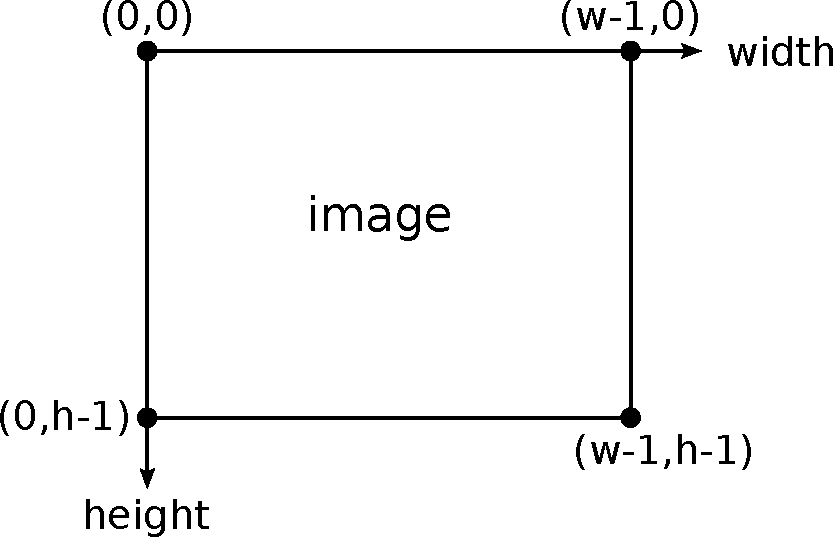
\includegraphics[scale=0.7]{figures/image_coord.pdf}
\caption{Image pixels coordinates}
\label{fig:image_coord}
\end{figure}

2D images can be defined with any positive w and h values. However, the real width and height will
always be respectively the smallest multiple of 64 greater than or equal to w and the smallest even
value greater than or equal to h. 

For instance, if you define an image (747x621), you will get a (768x622) image:

\lstset{language=Python}
\begin{lstlisting}
>>> im = imageMb(747, 621)
>>> im.getSize()
(768, 622) 
\end{lstlisting}

Two factors explain this particularity:

\begin{itemize}
\item In order to increase the processing speed, pixel values are stored in words and these
words may be 64 bits long if your OS allows it. By this means, 64 pixels of a binary image
are stored in a single word and then processed in parallel. The result is a dramatic increase
of the computation speed. So, if the horizontal size of the image is not multiple of 64, this could
deeply deteriorate the performance, as each end of line should be processed differently. 
\item Similarly, if the height is not even, a supplementary line is added to the image. The
reason is that the image can be processed on an hexagonal grid (see section \ref{cha:2Dgrids}). In this case and to
avoid again to increase the complexity of the operators, the number of even lines must be equal to
the number of odd ones.
\end{itemize}

The pixels added to the image are set to 0. This procedure is called padding. Padding may seem confusing
because it adds strips of black pixels on the right and bottom of the image. Therefore, processing such an
image leads to unwanted edge effects. The erosions for instance increase the size of the black strips
but many other operators are also concerned.

A better solution consists in cropping the image, that is cutting it in order to let it fit to the image size.
However, padding has been preferred to cropping because it allows the user not to lose any pixel of the image
and to choose at the end the part of it which will be discarded by cropping.

Nevertheless, cropping can be performed by two means:

\begin{itemize}
\item \textbf{cropCopy} can be used to extract from the padded image the part which interests you. Note that
\textbf{cropCopy} does not clear the destination image, it simply replace the cropped part (see the Mamba
Image Examples manual [\ref{art:MIEman}]).
\item The size of the destination image can also be set before loading the image file:

\lstset{language=Python}
\begin{lstlisting}
>>> im = imageMb(256, 256)
>>> im.load("myimage.png")
\end{lstlisting}

"myimage.png" is a (300x300) image stored in the Python working directory. This solution however does not allow you
to choose the part of the image which will be loaded: it is always the upper left part.
\end{itemize}

\subsection{3D images}
3D images are objects belonging to the \textbf{image3DMb} class. They inherit the attributes and methods of the
\textbf{imageMb} class. New attributes and methods are defined to deal with these images.

Basically, a Mamba 3D image is made of a pile of 2D images of same size and depth. The number of images in
the pile is given by the parameter \textit{length} and, contrary to the two other dimensions, there is no restriction
on the value of \textit{length}.

A 3D image is in fact a list of 2D images. Therefore, each 2D image at position \emph{i} (the indexing starts at 0) composing the 3D image im3D can
be accessed by:

\lstset{language=Python}
\begin{lstlisting}
im3D[i]
\end{lstlisting}

\begin{figure}
\centering
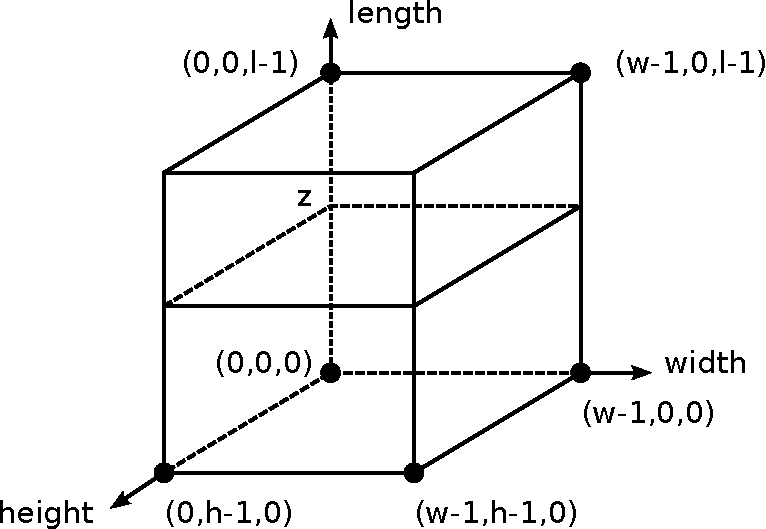
\includegraphics[scale=0.8]{figures/image3D_coord.pdf}
\caption{Image 3D pixels coordinates}
\label{fig:image3D_coord}
\end{figure}

Figure \ref{fig:image3D_coord} shows the coordinates arrangement of a 3D Mamba image. The length of the pile of 2D images (the third
dimension of the 3D image) corresponds to the length of the im3D list:

\lstset{language=Python}
\begin{lstlisting}
imLength = len(im3D)
\end{lstlisting}

Contrary to 2D images where a lot of formats are available, most of them being efficiently addressed by the
PILLOW library, there is not such standard formats in 3D. Many of them are proprietary. So, in Mamba 3D, there
exists only two ways to load a 3D image:

\begin{itemize}
\item By using the \textbf{loadRaw} method, where raw data are stored in the 3D image. Note that a preprocessing can
be performed on the data before loading them in the 3D image. See the Mamba Image User Manual [\ref{art:MIUman}]
and the Mamba Image Library Python Reference manual [\ref{art:MILPRman}] for further details. 
\item By using the \textbf{load} operator which reads a 3D image from a directory containing the corresponding pile
of 2D images.
\end{itemize}

Similarly, there are two procedures for saving 3D images:

\begin{itemize}
\item \textbf{extractRaw} extracts raw data from an image and stores them in a string. Then this string can be
written in a file.  
\item \textbf{save} stores all the 2D sections of the 3D image in a directory. This directory will contain 2D images
stored in a standard format.
\end{itemize}

\subsection{Sequences}
In the new release of Mamba (2.x), the \textbf{sequenceMb} class is simply an alias of the \textbf{image3DMb} class.
Indeed, a sequence is simply a list of 2D images. It can be considered as a special case of 3D image where
the third dimension is time.

\section{Grids}
Grids provide information on the neighborhood relationships between the pixels of an image.

A grid is not an attribute of the image. This point is very important and it is often disturbing as
displaying digitized images on a square grid (rectangular in fact) is quite common and lets believe that
the image is closely linked to the grid used to represent it, which is not true.

Conversely, a structuring element is always associated with a grid, otherwise it would be impossible
to define its geometry. More generally, a grid is associated to a morphological transformation. It is
indeed possible to define a given operator on different grids, but it is however very important to
know which grid we are working on. See the Mamba Image Library Coding Rules and Standards document [\ref{art:MILCRSman}] to
know the rules which must be enforced to avoid errors and mismatches when using the grids.

\subsection{2D grids}
\label{cha:2Dgrids}
Two grids are defined in 2D: the hexagonal and the square ones. 
The square grid defines 8 neighbors for each pixel and the hexagonal one, 6.

2D grids are built-in grids. There is no way to modify them (that is to modify the neighborhood
relationships) under Python. These grids are straightforward and you can see the coding of the directions
defined on these grids in the documentation (Mamba Image Library Python Reference [\ref{art:MILPRman}] and Mamba API
Quick Reference manual [\ref{art:MQRman}]).

On the hexagonal grid, an image contains even lines (\emph{h} coordinate multiple of 2) and odd lines. Even lines
are shifted to the left in relation to the odd lines, see figure \ref{fig:hex_grid}.
 
\begin{figure}
\centering
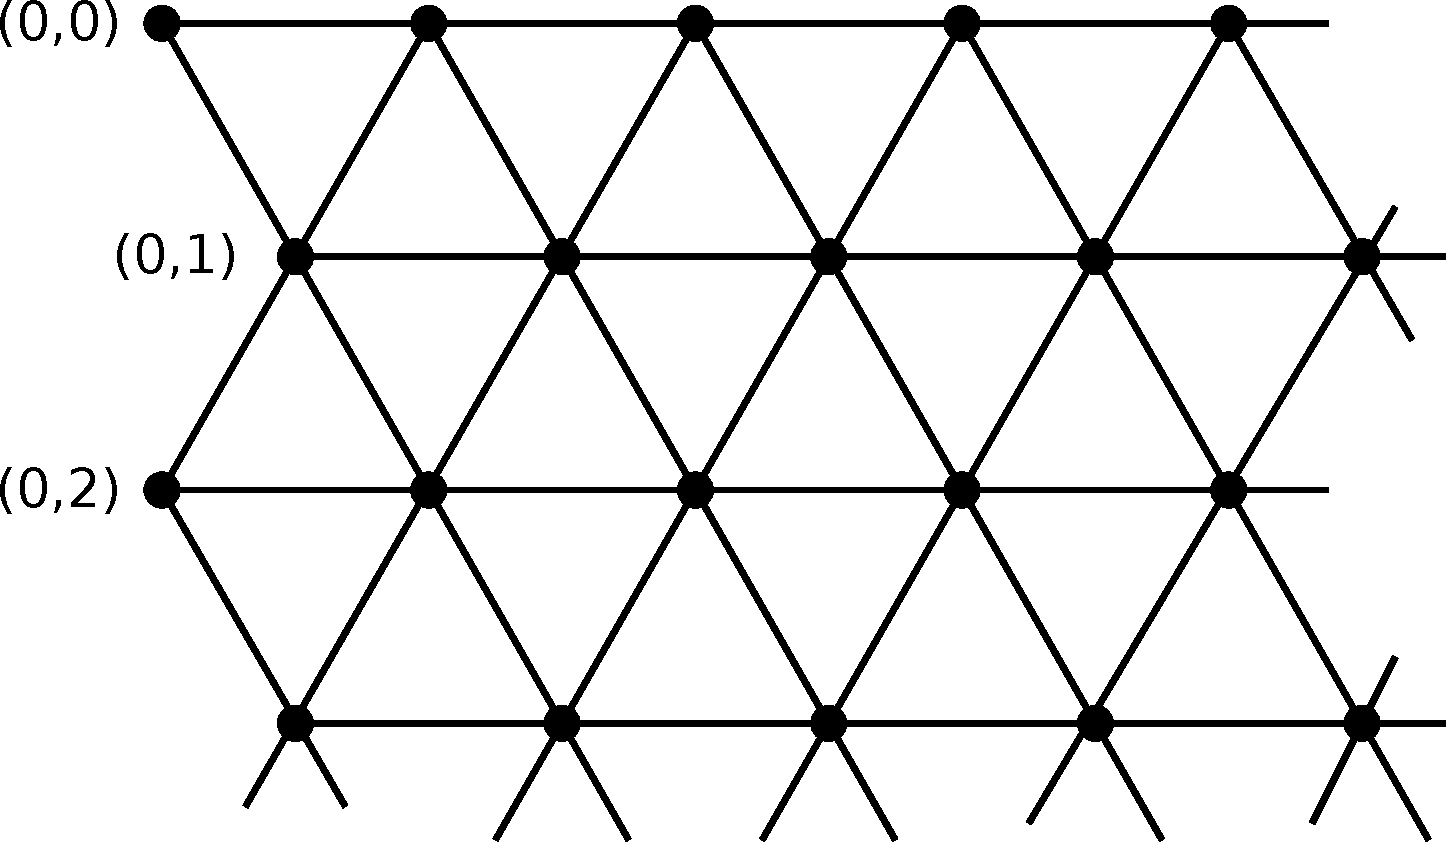
\includegraphics[scale=0.3]{figures/hex_grid.pdf}
\caption{Odd and even lines in the hexagonal grid}
\label{fig:hex_grid}
\end{figure}

Some public operators are available with 2D grids (which are instances of a class \textbf{\_grid}). They are self
explanatory. See the documentation on the directions encoding for further details.

\subsection{3D grids}
Grids in Mamba3D are defined in a more complex way. As 3D images can be considered as piles of 2D images,
a 3D grid is defined by providing two settings:

\begin{itemize}
\item The 2D grid (hexagonal or square) which is used with the 2D image sections of the 3D image.
\item The way these 2D images are stacked, this stacking defining the neighborhood relationships in the 3D grid.
\end{itemize}

Three grids are defined in Mamba3D: the Cubic grid (C), the Centered Cubic grid (CC) and the Face Centered Cubic grid (FCC),
see figure \ref{fig:3D_grids}.

\begin{figure}
\centering
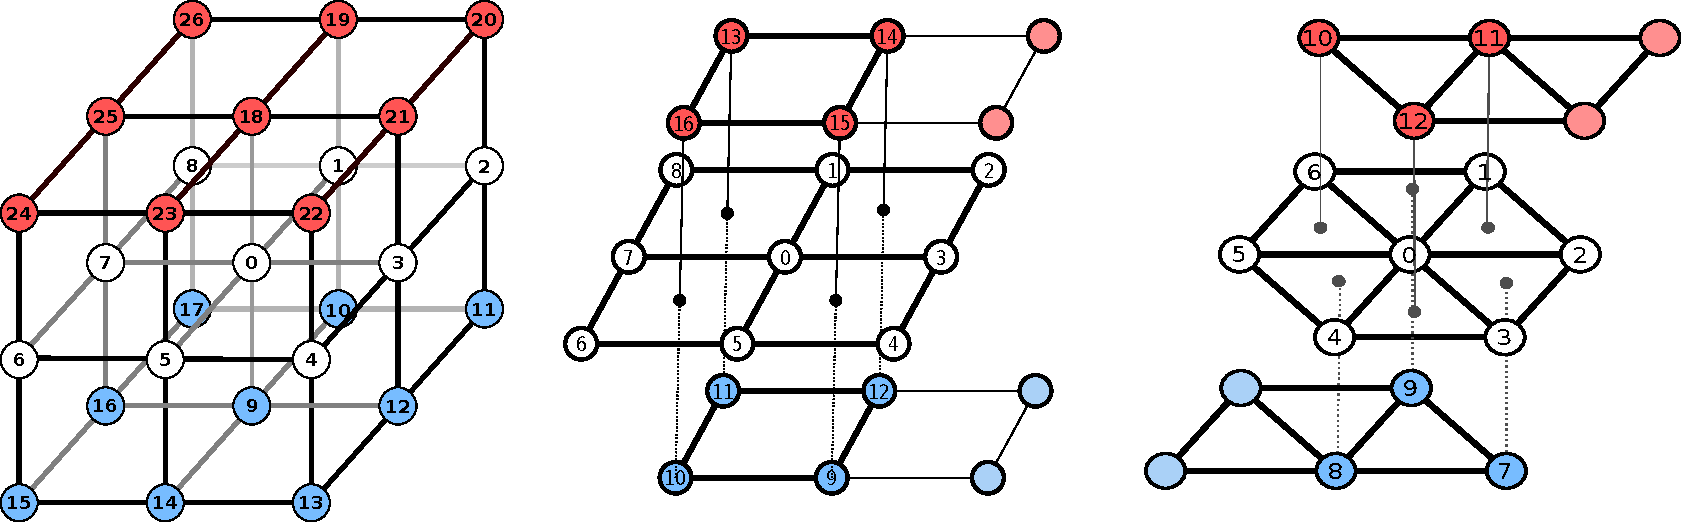
\includegraphics[scale=0.6]{figures/3D_grids.pdf}
\caption{3D grids defined in Mamba3D}
\label{fig:3D_grids}
\end{figure}

These grids are instances of a \textbf{\_grid3D} class. Each grid comes with various methods to handle it. Some of them are similar to
the operators provided with 2D grids. However, some others are specific and are more complex. These operators will be explicited
below for the different grids.

\subsubsection{Cubic grid}
This grid (named CUBIC) is made by stacking 2D images defined with a square grid.

For each 3D grid, The 2D grid on which it is based is given by the method \textbf{get2DGrid}:

\lstset{language=Python}
\begin{lstlisting}
>>> CUBIC.get2DGrid()
SQUARE
\end{lstlisting}

Each pixel of the cubic grid is surrounded by 26 neighbors, associated to 26 directions scattered among the section containing the
central pixel (8 directions) and the two sections below and above it (9 directions each). See the Mamba Image User Manual [\ref{art:MIUman}]
for the encoding of these directions.

Two interesting methods come with 3D grids: \textbf{getEncodedDirs} and \textbf{convertFromDir}.

\textbf{getEncodedDirs} is mainly used with 3D structuring elements. It allows to decompose any elementary 3D structuring element (defined
by a list of directions) into three 2D structuring elements corresponding to the three sections of the initial 3D structuring
element, see section \ref{cha:structelem} for further explanations.

\textbf{convertFromDir} requires two parameters: a 3D direction and the \emph{z} coordinate of the pixel. It returns a tuple containing the section
(-1 if below, 0 if current and 1 if above) and the 2D direction in this section corresponding to the 3D direction and to the \emph{z} position of the
pixel. We have for instance:

\lstset{language=Python}
\begin{lstlisting}
>>> CUBIC.convertFromdir(12, 5)
(-1, 3)
\end{lstlisting}

The direction 12 in the cubic grid corresponds to the direction 3 in the section below section 5.

Note that, for the cubic grid, the result is the same whatever \emph{z} because all the 2D images are stacked without shifting. It is
not the case for the other grids (see sections \ref{cha:CCgrid} and \ref{cha:FCCgrid}).

This method is quite useful to increase the computation speed of some 3D operators like shiftings as it provides directly
the \emph{z} offset and the corresponding horizontal direction (at least for the cubic grid - for the others, it is a bit more complex)
of this shifting.

\subsubsection{Centered cubic grid}
\label{cha:CCgrid}
Here again, this grid (named CENTER\_CUBIC) is defined by stacking 2D images defined with a square grid. But the odd sections
are shifted compared to the even sections just below so that the pixels be placed in the middle of the 2x2 squares of the below
section, hence the name "centered cubic". Therefore, this grid is made of an assembly of two shifted square grids which is
repeated all along the \emph{z} axis.

Figure \ref{fig:CC_grid} shows the relative arrangement of the odd and even planes.

\begin{figure}
\centering
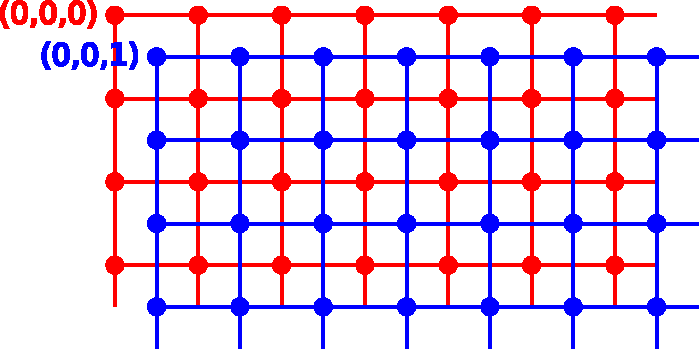
\includegraphics[scale=0.8]{figures/CC_grid.pdf}
\caption{Planes arrangement in the centered cubic grid}
\label{fig:CC_grid}
\end{figure}

Therefore, the \textbf{convertFromDir} operator returns a result which depends on the parity of the \emph{z} coordinate of the pixels:

\lstset{language=Python}
\begin{lstlisting}
>>> CENTER_CUBIC.convertFromdir(15, 0)
(1, 0)
>>> CENTER_CUBIC.convertFromdir(15, 1)
(1, 4)
\end{lstlisting}

Calculating the horizontal offsets in shifting operations is then more complicated as it depends of the relative parities
of the starting and ending planes.

\subsubsection{Face centered cubic grid}
\label{cha:FCCgrid}
The face centered cubic grid (named FACE\_CENTER\_CUBIC) is the most complex grid defined in Mamba3D. The 2D base grid is hexagonal
and the 3D grid is obtained by piling and shifting these 2D hexagonal grids.

In this case, three 2D hexagonal grids are used and shifted according to the scheme given in figure \ref{fig:FCC_grid}. Then, this configuration
is repeated along the \emph{z} axis.

\begin{figure}
\centering
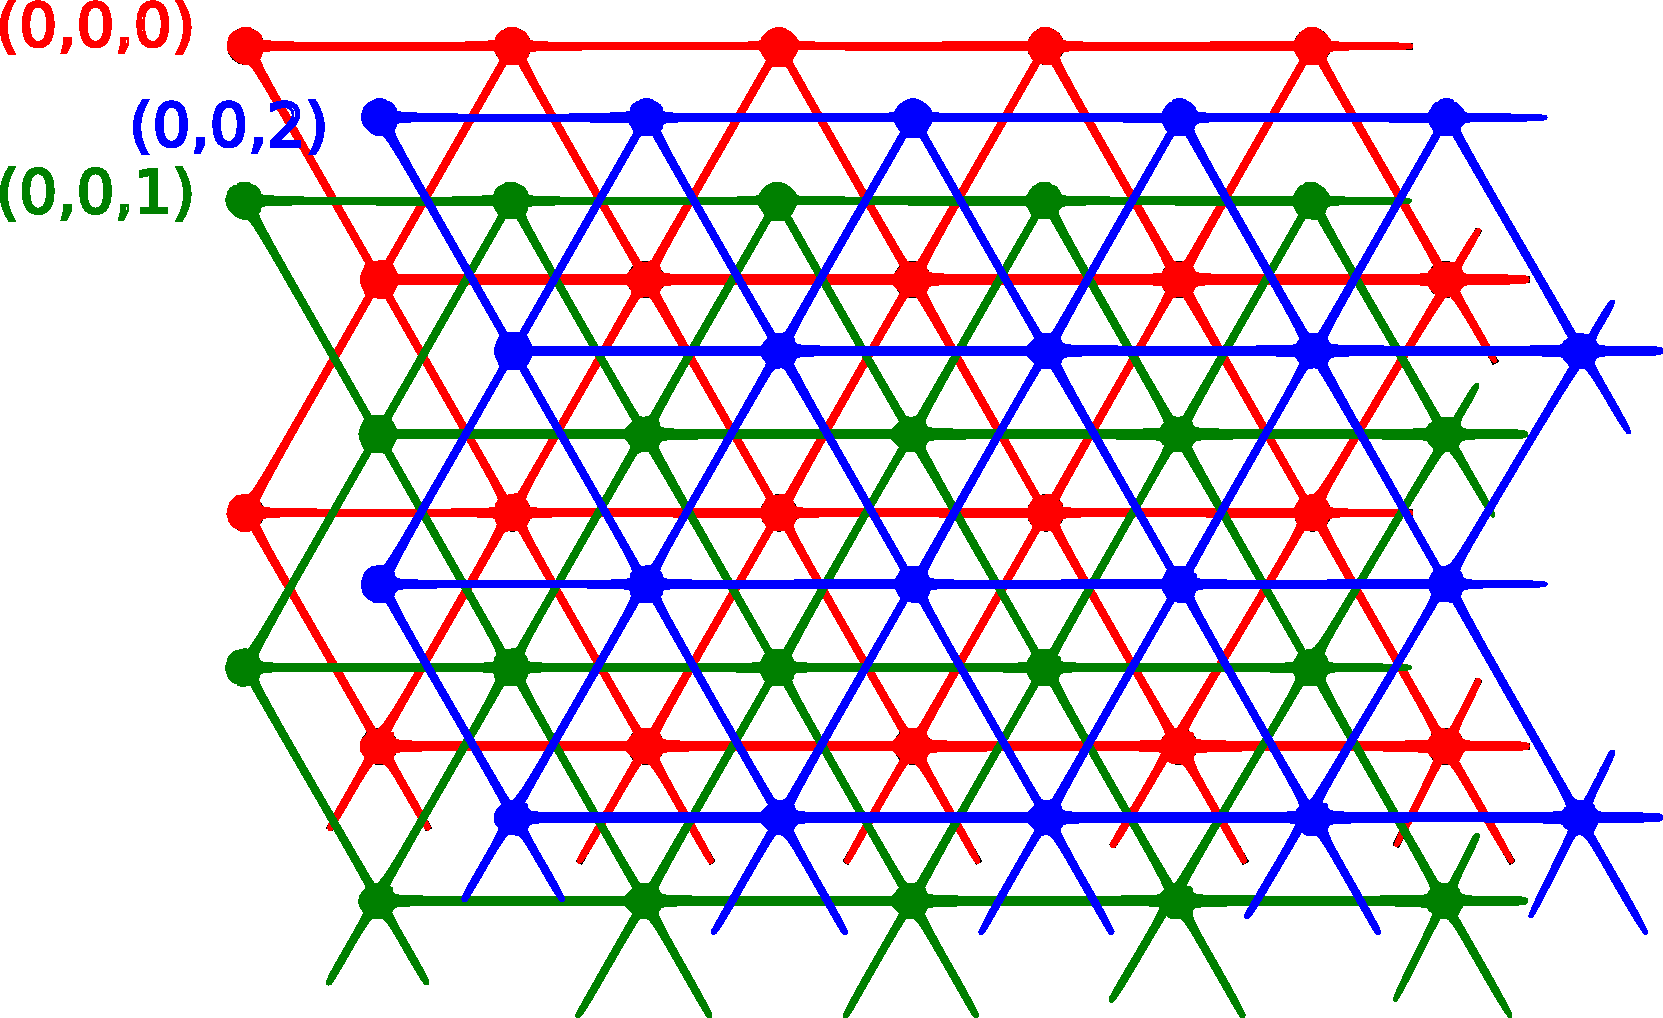
\includegraphics[scale=0.5]{figures/FCC_grid.pdf}
\caption{Planes arrangement in the face centered cubic grid}
\label{fig:FCC_grid}
\end{figure}

The \textbf{convertFromDir} operator provides different results according to the congruence modulo 3 of the \emph{z} coordinate with the values
0, 1 and 2:

\lstset{language=Python}
\begin{lstlisting}
>>> FACE_CENTER_CUBIC.convertFromdir(10, 0)
(1, 6)
>>> FACE_CENTER_CUBIC.convertFromdir(10, 1)
(1, 5)
>>> FACE_CENTER_CUBIC.convertFromDir(10, 2)
(1, 0)
\end{lstlisting}

Stacking and shifting 3 planes (instead of 2 as for the centered cubic grid) allows to define symmetrical structuring elements (cuboctahedrons).
Shifting only two planes would produce another grid structure named \textit{hexagonal closed packed} structure. Unfortunately, the structuring
elements defined on this grid are not symmetrical (we have in particular anticuboctahedrons).

\section{Edges}
Edges and edge management are very important in Mathematical Morphology, in particular (but not only) in  the definition of geodesic transforms.
Read the Mamba Image Library coding Rules and Standards manual [\ref{art:MILCRSman}] for explanations on edge settings for 2D images. Remind that,
in 2D, edges are virtual and not physically defined (there is no strip of pixels surrounding the images).

Edge management for 3D images is a combination of two approaches as edges in a 3D image are twofold. 3D images being made of a pile of 2D
images, the edges parallel to the \emph{z} axis are defined by the edges of the corresponding 2D images. These edges are therefore virtual and their management
is controlled by the \textit{edge} argument (set to EMPTY or FILLED) of the 2D images. But two other edges must be defined. They correspond
to the floor and the ceiling (along the \emph{z} axis) of the 3D volume of data formed by a 3D image. Contrary to the 2D edges, these two ones are
real and are built by adding two supplementary 2D images set to 0 or to the maximum value (1, 256 or $2^{32} - 1$) depending on the status (FILLED or EMPTY)
of the 2D edge (figure \ref{fig:3D_edges}).

\begin{figure}
\centering
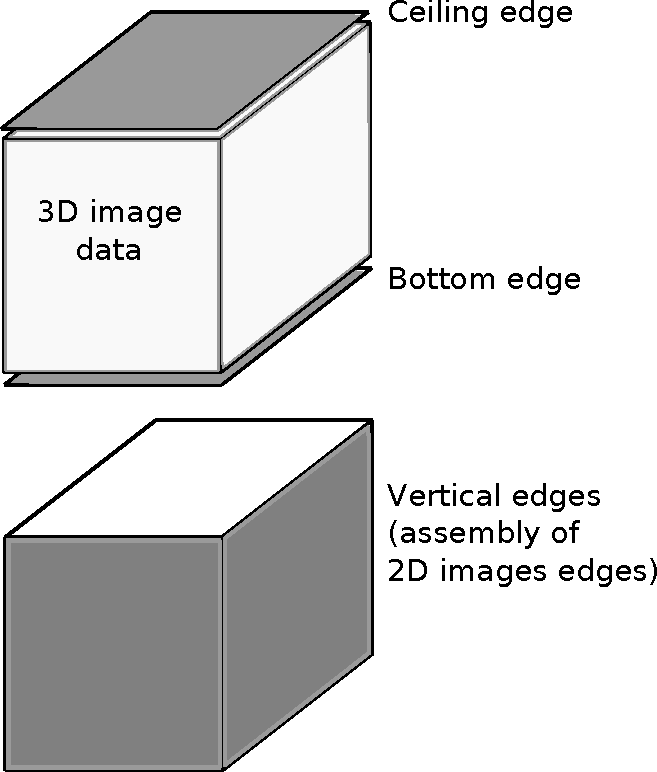
\includegraphics[scale=0.6]{figures/3D_edges.pdf}
\caption{Edges in a 3D image}
\label{fig:3D_edges}
\end{figure}

So, it is up to you, when defining operators where the edge status is relevant, to properly manage this status. As an example, have a look on the
definition of the erosions and dilations for 3D images.

Note that a method called \textbf{getZExtension} is associated with every defined grid. It returns an integer number corresponding to
the number of plans on each side of the central point which are needed to define all the neighbors of this point. All the currently
defined grids return 1 because all the neighbors are contained in the immediate planes below and above the central point. But more
sophisticated grids could be defined where the neighbors of the central point would belong to more than one plan apart. This parameter is
used for determining the number of top and bottom edge planes to be defined.
 
\section{Structuring elements}
\label{cha:structelem}
2D structuring elements are instances of the \textbf{structuringElement} class, while 3D ones are instances of the \textbf{structuringElement3D}
class. Remember also that a \textbf{doubleStructuringElement} and a \textbf{doubleStructuringElement3D} classes exist. They are used with
the thinning and thickening operators.
Each structuring element is associated to a grid. It is defined by the neighbors of the central point it contains. Its origin is always
the central point, even when this point does not belong to the structuring element. Different methods exist to deal with these 2D and
3D structuring elements: \textbf{getGrid} returns the grid associated with the structuring element, \textbf{getDirections} returns the
directions used by the structuring element (with or without direction 0), \textbf{hasZero} indicates if the structuring element contains
or not the central point, etc.
In 2D, a major difference between Mamba 1.x and Mamba 2.x lies in the way directions are defined and used in the \textbf{infNeighbor}, \textbf{supNeighbor}
and \textbf{diffNeighbor} operators. It is now possible to use several directions at the same time. These directions, however, must be coded.
This coding is performed by the \textbf{getEncodedDirections} method. All the directions \emph{i} of the structuring element \emph{se} are used to define a
number \emph{nb} equal to:

\begin{displaymath}
nb = \sum_{i \in se} 2^i
\end{displaymath}

which is actually used by the operators. The main advantage of this approach is a dramatic increase of the computation speed of the basic
morphological transforms (erosion, dilation). Here are examples of direction encoding for some common structuring elements:

\lstset{language=Python}
\begin{lstlisting}
>>> HEXAGON.getEncodedDirections()
127
>>> HEXAGON.getEncodedDirections(withoutZero=True)
126
>>> TRIANGLE.getEncodedDirections()
25
\end{lstlisting}

In 3D, the same encoding is needed. But, as the structuring elements can be defined on three 2D layers, this encoding is performed on each
one so that the basic 3D erosions and dilations can be obtained rapidly by performing partial operations on each plane of the 3D image and by
combining these partial results. This encoding is performed by the \textbf{getEncodedDirs} method which returns a dictionnary containing the 2D
structuring elements encodings for the three sections of a given 3D structuring element. The result obviously depends of the \emph{z} position of the
structuring element:

\lstset{language=Python}
\begin{lstlisting}
>>> dirs = CUBOCTAHEDRON1.getDirections()
>>> CUBOCTAHEDRON1.grid.getEncodedDirs(dirs, 0)
{0: 127, 1: 67, -1: 97}
>>> CUBOCTAHEDRON1.grid.getEncodedDirs(dirs, 1)
{0: 127, 1: 49, -1: 25}
>>> CUBOCTAHEDRON1.grid.getEncodedDirs(dirs, 2)
{0: 127, 1: 13, -1: 7}
\end{lstlisting}

\section{References}
\begin{enumerate}
\setcounter{enumi}{0}
\item \label{art:MILCRSman} Nicolas Beucher and Serge Beucher,
\emph{Mamba Image Library Coding Rules and Standards},
Mamba documentation available at \url{http://www.mamba-image.org}.
\item \label{art:MIUman} Nicolas Beucher and Serge Beucher,
\emph{Mamba Image User Manual},
Mamba documentation available at \url{http://www.mamba-image.org}.
\item \label{art:MIEman} Nicolas Beucher and Serge Beucher,
\emph{Mamba Image Examples},
Mamba documentation available at \url{http://www.mamba-image.org}.
\item \label{art:MILPRman} Nicolas Beucher and Serge Beucher,
\emph{Mamba Image Library Python Reference},
Mamba documentation available at \url{http://www.mamba-image.org}.
\item \label{art:MQRman} Nicolas Beucher,
\emph{Mamba API Quick Reference},
Mamba documentation available at \url{http://www.mamba-image.org}.
\end{enumerate}

\end{document}




